\documentclass[11pt,twoside]{article}
%\usepackage{etex}

\raggedbottom

%geometry (sets margin) and other useful packages
\usepackage{geometry}
\geometry{top=1in, left=1in,right=1in,bottom=1in}
 \usepackage{graphicx,booktabs,calc}
 
\usepackage{listings}


% Marginpar width
%Marginpar width
\newcommand{\pts}[1]{\marginpar{ \small\hspace{0pt} \textit{[#1]} } } 
\setlength{\marginparwidth}{.5in}
%\reversemarginpar
%\setlength{\marginparsep}{.02in}

 
%\usepackage{cmbright}lstinputlisting
%\usepackage[T1]{pbsi}


\usepackage{chngcntr,mathtools}
\counterwithin{figure}{section}
\numberwithin{equation}{section}

%\usepackage{listings}

%AMS-TeX packages
\usepackage{amssymb,amsmath,amsthm} 
\usepackage{bm}
\usepackage[mathscr]{eucal}
\usepackage{colortbl}
\usepackage{color}


\usepackage{subfigure,hyperref,enumerate,polynom,polynomial}
\usepackage{multirow,minitoc,fancybox,array,multicol}

\definecolor{slblue}{rgb}{0,.3,.62}
\hypersetup{
    colorlinks,%
    citecolor=blue,%
    filecolor=blue,%
    linkcolor=blue,
    urlcolor=slblue
}

%%%TIKZ
\usepackage{tikz}

\usepackage{pgfplots}
\pgfplotsset{compat=newest}

\usetikzlibrary{arrows,shapes,positioning}
\usetikzlibrary{decorations.markings}
\usetikzlibrary{shadows}
\usetikzlibrary{patterns}
%\usetikzlibrary{circuits.ee.IEC}
\usetikzlibrary{decorations.text}
% For Sagnac Picture
\usetikzlibrary{%
    decorations.pathreplacing,%
    decorations.pathmorphing%
}

\tikzstyle arrowstyle=[black,scale=2]
\tikzstyle directed=[postaction={decorate,decoration={markings,
    mark=at position .65 with {\arrow[arrowstyle]{stealth}}}}]
\tikzstyle reverse directed=[postaction={decorate,decoration={markings,
    mark=at position .65 with {\arrowreversed[arrowstyle]{stealth};}}}]
\tikzstyle dir=[postaction={decorate,decoration={markings,
    mark=at position .98 with {\arrow[arrowstyle]{latex}}}}]
\tikzstyle rev dir=[postaction={decorate,decoration={markings,
    mark=at position .98 with {\arrowreversed[arrowstyle]{latex};}}}]

\usepackage{ctable}

%
%Redefining sections as problems
%
\makeatletter
\newenvironment{exercise}{\@startsection 
	{section}
	{1}
	{-.2em}
	{-3.5ex plus -1ex minus -.2ex}
    	{1.3ex plus .2ex}
    	{\pagebreak[3]%forces pagebreak when space is small; use \eject for better results
	\large\bf\noindent{Exercise 1.\hspace{-1.5ex} }
	}
	}
	%{\vspace{1ex}\begin{center} \rule{0.3\linewidth}{.3pt}\end{center}}
	%\begin{center}\large\bf \ldots\ldots\ldots\end{center}}
\makeatother

%
%Fancy-header package to modify header/page numbering 
%
\usepackage{fancyhdr}
\pagestyle{fancy}
%\addtolength{\headwidth}{\marginparsep} %these change header-rule width
%\addtolength{\headwidth}{\marginparwidth}
%\fancyheadoffset{30pt}
%\fancyfootoffset{30pt}
\fancyhead[LO,RE]{\small Oke}
\fancyhead[RO,LE]{\small Page \thepage} 
\fancyfoot[RO,LE]{\small PS 1} 
\fancyfoot[LO,RE]{\small \scshape CEE 260/MIE 273} 
\cfoot{} 
\renewcommand{\headrulewidth}{0.1pt} 
\renewcommand{\footrulewidth}{0.1pt}
%\setlength\voffset{-0.25in}
%\setlength\textheight{648pt}


\usepackage{paralist}

\newcommand{\osn}{\oldstylenums}
\newcommand{\lt}{\left}
\newcommand{\rt}{\right}
\newcommand{\pt}{\phantom}
\newcommand{\tf}{\therefore}
\newcommand{\?}{\stackrel{?}{=}}
\newcommand{\fr}{\frac}
\newcommand{\dfr}{\dfrac}
\newcommand{\ul}{\underline}
\newcommand{\tn}{\tabularnewline}
\newcommand{\nl}{\newline}
\newcommand\relph[1]{\mathrel{\phantom{#1}}}
\newcommand{\cm}{\checkmark}
\newcommand{\ol}{\overline}
\newcommand{\rd}{\color{red}}
\newcommand{\bl}{\color{blue}}
\newcommand{\pl}{\color{purple}}
\newcommand{\og}{\color{orange!90!black}}
\newcommand{\gr}{\color{green!40!black}}
\newcommand{\nin}{\noindent}
\newcommand{\la}{\lambda}
\renewcommand{\th}{\theta}
\newcommand*\circled[1]{\tikz[baseline=(char.base)]{
            \node[shape=circle,draw,thick,inner sep=1pt] (char) {\small #1};}}

\newcommand{\bc}{\begin{compactenum}[\quad--]}
\newcommand{\ec}{\end{compactenum}}

\newcommand{\n}{\\[2mm]}
%% GREEK LETTERS
\newcommand{\al}{\alpha}
\newcommand{\gam}{\gamma}
\newcommand{\eps}{\epsilon}
\newcommand{\sig}{\sigma}

\newcommand{\p}{\partial}
\newcommand{\pd}[2]{\frac{\partial{#1}}{\partial{#2}}}
\newcommand{\dpd}[2]{\dfrac{\partial{#1}}{\partial{#2}}}
\newcommand{\pdd}[2]{\frac{\partial^2{#1}}{\partial{#2}^2}}
\newcommand{\mr}{\mathbb{R}}
\newcommand{\xs}{x^{*}}
\newenvironment{solution}
{\medskip\par\quad\quad\begin{minipage}[c]{.8\textwidth}\gr}{\medskip\end{minipage}}

 
%%%%%%%%%%%%%%%%%%%%%%%%%%%%%%%%%%%%%%%%%%%%%%%%%%%
%%%%%%%%%%%%%%%%%%%%%%%%%%%%%%%%%%%%%%%%%%%%%%%%%%%

\begin{document}

\lstset{language=C++,
                basicstyle=\tiny\ttfamily,
                keywordstyle=\color{blue}\ttfamily,
                stringstyle=\color{red}\ttfamily,
                commentstyle=\color{gray}\ttfamily,
                morecomment=[l][\color{gray}]{\#}
}


\thispagestyle{empty}


\nin{\LARGE Problem Set 1 {\gr }}\hfill{\bf Prof. Oke}

\medskip\hrule\medskip

\nin {\small CEE 260/MIE 273: Probability \& Statistics in Civil Engineering
\hfill\textit{ 09.04.2025}}

\bigskip

\nin{\it Due Tuesday, September 15, 2026 at 12:59 PM as PDF uploaded via Gradescope.
Submit your file as a PDF. There are 3 problems, with a total of 17 points. 
}\\


\section*{Problem 1 \textit{(5 points)}}

Respond ``T'' ({\it True})  or  ``F'' (\textit{False}) to the following statements. Use the boxes provided. Each response is worth 1 point.

\begin{enumerate}[\bf (i)]
\item \hfill
  \begin{minipage}{.1\linewidth}
    \framebox(40,40){ \gr }
  \end{minipage}\quad
  \begin{minipage}{.85\linewidth}
    The standard deviation of a random sample is a measure of its central tendency. %False
  \end{minipage}
%  \underline{\hspace{10ex}} %F 

    \smallskip

% \item \hfill
%   \begin{minipage}{.1\linewidth}
%     \framebox(40,40){\gr T}
%   \end{minipage}\quad
%   \begin{minipage}{.85\linewidth}
%     Clustering is a supervised learning approach. %False
%   \end{minipage}

%   \smallskip
  
\item \hfill
  \begin{minipage}{.1\linewidth}
    \framebox(40,40){\gr }
  \end{minipage}\quad
  \begin{minipage}{.85\linewidth}
    In a perfectly symmetric distribution, the median is equal to the mean. %True
  \end{minipage}

  \smallskip
  
\item \hfill
  \begin{minipage}{.1\linewidth}
    \framebox(40,40){\gr }
  \end{minipage}\quad
  \begin{minipage}{.85\linewidth}
    A right-skewed distribution has a long left tail. %False
  \end{minipage}

  \smallskip
  
\item \hfill
  \begin{minipage}{.1\linewidth}
    \framebox(40,40){\gr }
  \end{minipage}\quad
  \begin{minipage}{.85\linewidth}
    In a boxplot (introduced in 1970 by John Tukey), the whiskers are conventionally selected as the values closest to within
    $Q_{1} - 1.5IQR$ and $Q_{3}+1.5IQR$.
    In this case, the distance between the whiskers is $4IQR$. %True
  \end{minipage}

  
  \smallskip
  
\item \hfill
  \begin{minipage}{.1\linewidth}
    \framebox(40,40){\gr }
  \end{minipage}\quad
  \begin{minipage}{.85\linewidth}
    The mean of a sample dataset can be determined from its boxplot. %False
  \end{minipage}
  
  \smallskip
  
% \item \hfill
%   \begin{minipage}{.1\linewidth}
%     \framebox(40,40){\gr }
%   \end{minipage}\quad
%   \begin{minipage}{.85\linewidth}
%    Given $A$ and $B$ are two mutually exclusive events. $A \cap B = \varnothing$. %True
%   \end{minipage}
  \end{enumerate}

  % \smallskip
  
% \item \hfill
%   \begin{minipage}{.1\linewidth}
%     \framebox(40,40){}
%   \end{minipage}\quad
%   \begin{minipage}{.85\linewidth}
%     A good clustering solution should maximize the total within-cluster variation. %False
%   \end{minipage}

\eject  
\section*{Problem 2 \textit{(2 points)}}
How would you describe the relationship between the variables shown in each of the following plots? Indicate the correct answer in each case (by circling, or otherwise).

\begin{enumerate}[\bf (a)]
\item ~\pts{1}
  \begin{figure}[h!]
    \centering
    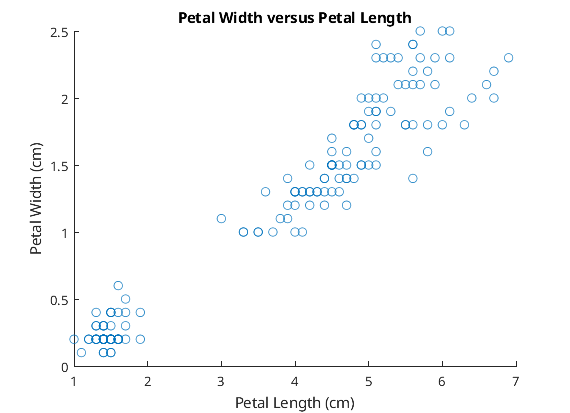
\includegraphics[width=.5\textwidth]{pwpl}
  \end{figure}

  \begin{enumerate}[\bf (i)]
  \item{Approximately linear}
  \item Nonlinear
  \item No discernible relationship
  \end{enumerate}

  \bigskip
  
\item  ~ \pts{1}
  \begin{figure}[h!]
    \centering
    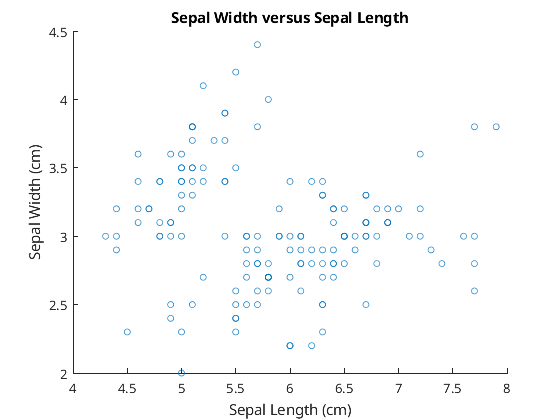
\includegraphics[width=.5\textwidth]{swsl}
  \end{figure}

    \begin{enumerate}[\bf (i)]
  \item Approximately linear
  \item Nonlinear
  \item No discernible relationship
  \end{enumerate}
\end{enumerate}

  \eject

 %  \section*{Problem 3 \textit{(6 points)}}
  
 % Open Into, Exercise 1.40 (Income and education in US counties, p. 37) \pts{6}
  


 %   \vspace{25ex}

 %   \eject
   
\section*{Problem 3 \textit{(10 points)}}
You are given a sample of 43 beak sizes ($X$) measured from a certain bird species on an island.
The sample  mean $\ol X$ is 10.77 mm and the sample variance $s^{2} = 1.048$. The median $m$ is 10.65 mm.
\begin{enumerate}[\bf (a)]
\item Find the sample standard deviation $s$ of the dataset.\pts{2}
   \vspace{18ex}

\item Find the sampling error (also known as the standard error of the mean, $SE$). \pts{2}
   \vspace{18ex}


\item Find the coefficient of variation $\delta_{X}$. \pts{2}
   \vspace{18ex}

\item The first and third  quartiles of the sample are given by $Q_{1} = 10.2175, Q_{3} = 11.22$.
  \begin{enumerate}[\bf (i)]
  \item What is the second \pts{1} quartile? %$\gr \boxed{Q_{2} = m = 10.65}$
   \bigskip
   \bigskip
    
  \item Find the interquartile range (IQR) of the sample.\pts{1}
   \vspace{12ex}

  \end{enumerate}

\item The maximum value of the sample is 13.49 mm. \pts{2} If a boxplot is constructed with the whiskers determined by $Q_{1} - 1.5IQR$ and $Q_{3}+1.5IQR$, would you expect to see any outliers in the plot? Explain briefly.

     \vspace{25ex}

\end{enumerate}


% \section*{Problem 4 \textit{(8 points)}}
% Exercise 1.44 (Space Launches), Open Intro textbook.

% \section*{Problem 5 \textit{12 points}}
% Exercise 2.16 (Distributions and appropriate statistics, Part II)

% \section*{Problem 6 \textit{}}
% To be provided by Wednesday.
   
\end{document}


%%% Local Variables:
%%% mode: latex
%%% TeX-master: t
%%% End:
